\chapter{Επαλήθευση Λειτουργίας και Αποτελέσματα} % Main chapter title
\label{chap:Chapter6}

% \epigraph{”Testing a product is a learning process"}{\textit{Brian Mahick}}
\epigraph{”Η διαδικασία δοκιμών ενός συστήματος είναι μία διαδικασία εκμάθησης''}{\textit{Brian Mahick}}

Σε αυτό το σημείο περιγράφονται οι ενέργειες που ακολουθήθηκαν, προκειμένου να επαληθευτεί η απόδοση του συστήματος.
Η διαδικασία δοκιμών χωρίστηκε σε τρία στάδια. Το πρώτο, το οποίο γινόταν σε indoor περιβάλλον ταυτόχρονα με την υλοποίηση του συστήματος
ώστε να επαληθευτεί η δυνατότητα εντοπισμού της μπάλας σε κάθε frame του feed της κάμερας\footnote{Βίντεο από την διαδικασία μπορεί να βρεθεί \cite{experiment-1-video}}. Την δεύτερη
που αποτελεί το κομμάτι δοκιμών ενός μεμονωμένου node σε outdoor scenarios για το localization στο image plane του αντικειμένου με βάση την μέθοδο εντοπισμού που επιλέχθηκε\footnote{
Βίντεο από την διαδικασία μπορεί να βρεθεί \cite{experiment-2-video}}. Τελευταίο κομμάτι ήταν η δοκιμή ολόκληρου του συστήματος\footnote{Βίντεο από την διαδικασία μπορεί να βρεθεί \cite{TODO}}.

Στην συνέχεια του κεφαλαίου, δίνονται αναλυτικά στοιχεία για την δεύτερη και τρίτη φάση δοκιμών και όχι για την πρώτη, καθώς περιλαμβάνονται σε αυτές μετρικές της πρώτης. Ενώ, για την ανίχνευση του object στο εκάστοτε καρέ χρησιμοποιείται η διαδικασία με τον HSV μετασχηματισμό (βλ. \Sect{hsv-detection-sec}).

Ο λόγος επιλογής της HSV μεθόδου στην συγκεκριμένη εργασία είναι ότι μπορεί να παρέχει ικανοποιητική απόδοση όντως πρώτη γενιά του συστήματος - με μικρές σχετικά ανάγκες επεξεργασίας - παρόλα αυτά, κύριο αρνητικό της είναι η ανάγκη πριν την χρήση του συστήματος να πραγματοποιηθεί calibration.

\section{Επαλήθευση λειτουργίας μεμονωμένου node}

\subsection{Περιβάλλον δοκιμών}
Για την επαλήθευση λειτουργίας του μεμονωμένου κόμβου, η διαδικασία που ακολουθήθηκε είναι η εξής. 
Χρησιμοποιήθηκαν δύο αντικείμενα, το υπό έλεγχο σύστημα - \Fig{node-testing-env} (a) - το οποίο κατά όλη την διάρκεια του πειράματος ήταν στατικό σε συγκεκριμένο σημείο, και το κινούμενο αντικείμενου (η κίτρινη μπάλα), η θέση του οποίου έγινε προσπάθεια κάθε χρονική στιγμή να εκτιμηθεί - \Fig{node-testing-env} (b).   

\begin{figure} [H]
	\centering
	% -----------------
    \begin{minipage}{.5\textwidth}
      \centering
      \includegraphics[width=\linewidth, angle =-90]{../Images/Experiments-Results/node.jpg} \\ \vspace{0.1cm}
      {(a) Υπό έλεγχο σύστημα (Node) το οποίο τροφοδοτείται από powerbank κατά την διάρκεια πειραμάτων}
    \end{minipage}%
    % -----------------
    \begin{minipage}{.5\textwidth}
      \centering
      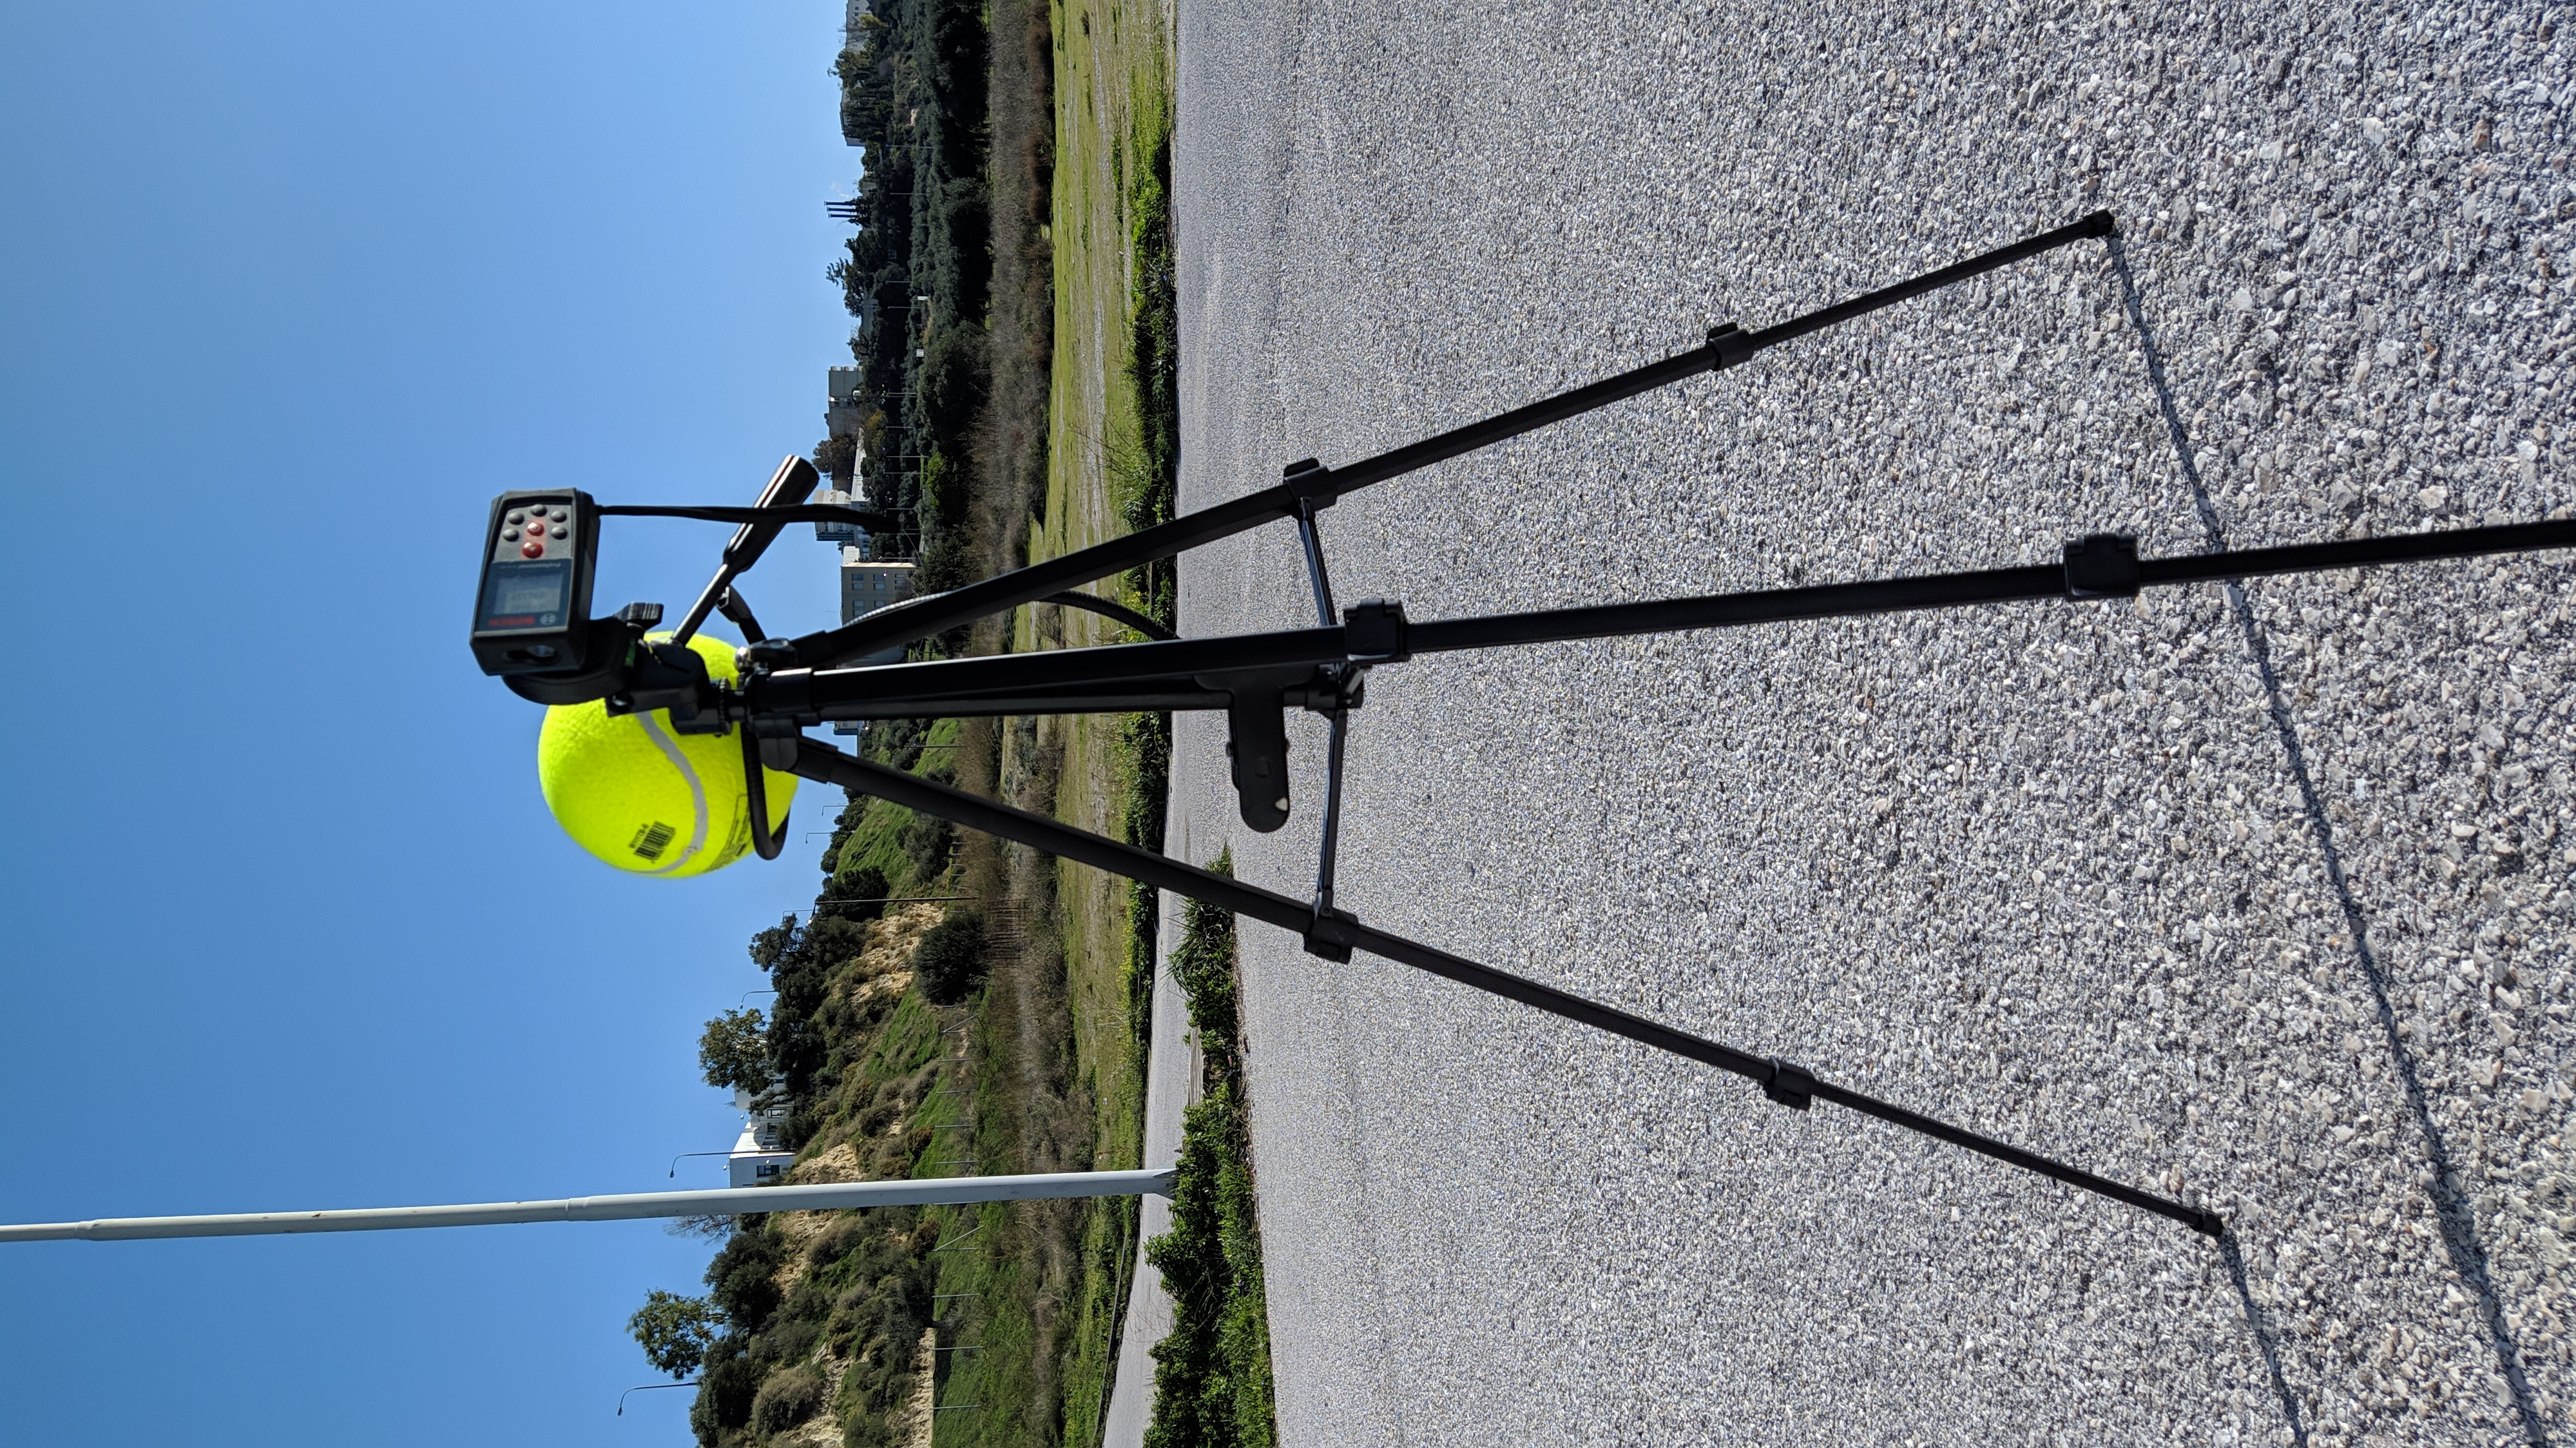
\includegraphics[width=\linewidth, angle =-90]{../Images/Experiments-Results/testing.jpg}\\ \vspace{0.1cm}
      {(b) Κινούμενο αντικείμενο εκτίμησης θέσης μαζί με το όργανο μέτρησης απόστασης }
	\end{minipage}
	% -----------------
    \hfill \break
    \decoRule
    \CaptionBasedwithURL{Εξοπλισμός που χρησιμοποιήθηκε στην πρώτη εξωτερική πειραματική φάση} 
    \label{fig:node-testing-env}
\end{figure}

Τα δύο αυτά αντικείμενα τοποθετήθηκαν το ένα απέναντι από το άλλο όπως φαίνεται στην \Fig{single-test-bench-side-view}, και πάρθηκαν μετρήσεις απόστασης για διαφορετικές γωνίες όπως φαίνεται στην 
\Fig{single-test-bench-angles}. Ταυτόχρονα, το σύστημα κατά την διάρκεια της διαδικασίας, ήταν σε πλήρη λειτουργία, και πραγματοποιούσε ανίχνευση και εκτίμηση της απόστασης του αντικειμένου από την κάμερα. Στη
\Sect{expe-single-3d} παρουσιάζονται τα πειραματικά αποτελέσματα των μετρήσεων αυτής της διαδικασία, ενώ στη 
\Sect{single-expe-system} παρουσιάζονται οι ανάγκες λειτουργίας από την σκοπιά του ε\-νσω\-μα\-τω\-μέ\-νου συστήματος.

\FigCaptLabelBasedURL{../Images/Experiments-Results/side.jpg}
{Χωρική τοποθέτηση του υπό ελέγχου συστήματος και αντικειμένου εκτίμησης θέσης}%
{single-test-bench-side-view}%
<0.8>

\FigCaptLabelBasedURL{../Images/Experiments-Results/testbench.png}
{Αναπαράσταση των θέσεων στις οποίες έγιναν οι μετρήσεις του πειράματος}%
{single-test-bench-angles}%
<0.6>

Όπως φαίνεται στην \Fig{node-testing-env} (b), το object το οποίο πρόκειται να εντοπίσουμε βρίσκεται σε τρίποδο, για μεγαλύτερη ευκολία των μετρήσεων, ενώ στο πλάγιο μέρος γίνεται διακριτό το όργανο που χρησιμοποιήθηκε για τον υπολογισμό της απόστασης μεταξύ των δύο αντικειμένων. Το όργανο αυτό είναι το laser range finder της Bosch GLM 40 - \Fig{bosch-range-estimator} - με δυνατότητες μέτρησης $0.15-40.00 m$ και απόκλιση μετρήσεων $\pm1.5mm$

Για τον υπολογισμό των διάφορων γωνιών από τις οποίες θα γινόντουσαν μετρήσεις, χρησιμοποιήθηκε το όργανο μέτρησης γωνιών όπως φαίνεται στην \Fig{single-test-bench-top-view}. Ενώ οι μετρήσεις που στην συνέχεια θα αναγερθούν αφορούν δεδομένα από γωνίες [$-20\si{\degree},-10\si{\degree},~0\si{\degree},~10\si{\degree},~20\si{\degree}$]\footnote{Λόγω του διαφορετικού ύψους μεταξύ της θέσης που μετρήθηκαν οι γωνίες και της κάμερας, δεν είναι οι ίδιες με αυτές που ανιχνεύονται στο x άξονα της εικόνας}.

\FigCaptLabelBasedURL{../Images/Experiments-Results/glm40.jpg}
{Το ψηφιακό λέιζερ μέτρησης απόστασης που χρησιμοποιήθε (Bosch GLM 40)}%
{bosch-range-estimator}%
<0.4>%
(https://www.howetools.co.uk/bosch-glm-40-aaa-batteries-laser-range-finder)

\FigCaptLabelBasedURL{../Images/Experiments-Results/node-top-view.jpg}
{Υπολογισμός των γωνιών με χρήση εργαλείου μέτρησης γωνίας}%
{single-test-bench-top-view}%
<0.9>

% -------------------------------------------------------------
\subsection{Απόδοση του συστήματος} \label{sec:single-expe-system}

Πριν αναφερθούν τα δεδομένα που συλλέχθηκαν ως προς την απόδοση του συστήματος, θα αναφερθούν κάποια από τα 
χαρακτηριστικά λειτουργίας του. Η υλοποίηση του συστήματος έγινε σε C++. Δημιουργήθηκαν συνεπώς Function-like macros για εξαγωγή και αποθήκευση χρήσιμων πληροφοριών του συστήματος. Οι πληροφορίες που συλλέχθηκαν, αναφέρονται σε αυτήν την ενότητα, και σχετίζονται με τις επεξεργαστικές και ενεργειακές ανάγκες του συστήματος, η μνήμη μου χρειάζεται για να λειτουργήσει, και άλλες σημαντικές πληροφορίες.

Πρώτη από αυτές τις πληροφορίες είναι οι επεξεργαστικές ανάγκης του, όπου στην \Fig{cpu-usage-experiment-example}
φαίνονται τα δεδομένα που συλλέχθηκαν κατά την διάρκεια ενός από τα πειράματα. 

\FigCaptLabelBasedURL{../Images/Experiments-Results/raspberry-exp-cpu.png}
{Επεξεργαστική ισχύς του συστήματος}%
{cpu-usage-experiment-example}%
<1>

Μία ακόμα χρήσιμη μετρική είναι αυτή της μνήμης που χρησιμοποιεί το σύστημα, στην \Fig{ram-usage-experiment-example}
παρουσιάζεται η συγκεκριμένη πληροφορία. Από αυτό το διάγραμμα μπορούμε να παρατηρήσουμε ότι για την συγκεκριμένη υλοποίηση το σύστημα δεν έχει μεγάλες ανάγκες μνήμης\footnote{Έχοντας αυτήν την πληροφορία, μπορούμε να μεταβούμε σε επιλογή embedded linux system με μικρότερη μνήμη, που σημαίνει μικρότερο κόστος ανά node συστήματος}.
\FigCaptLabelBasedURL{../Images/Experiments-Results/raspberry-exp-ram.png}
{Ανάγκες μνήμης του συστήματος}%
{ram-usage-experiment-example}%
<1>

Το σύστημα αυτό σχεδιάζεται, με γνώμονα μελλοντικά να χρησιμοποιηθεί σε drones, συνεπώς οι ενεργειακές απαιτήσεις του είναι σημαντικές. Για αυτό τον λόγο ε\-ξά\-χθη\-καν και δεδομένα σχετικά με την κατανάλωση του συστήματος\footnote{Στις συγκεκριμένες γραφικές, μέχρι το 80s το σύστημα είναι σε idle mode, ενώ από εκεί και έπειτα είναι σε πλήρη λειτουργία} - \Fig{power-usage-experiment-example}. Με την μέγιστη κατανάλωση που παρατηρήθηκε από τροφοδοσία μέσω power bank κατά την διάρκεια δοκιμών είναι τα 10Watt, ενώ τάση τροφοδοσίας είναι τα 5Volt.
\FigCaptLabelBasedURL{../Images/Experiments-Results/raspberry-exp-power.png}
{Ενεργιακές απαιτήσεις συστήματος}%
{power-usage-experiment-example}%
<1>

Σημαντικός παράγοντας της απόδοσης ενός επεξεργαστή, είναι η θερμοκρασία του, καθώς αν είναι αυξημένη μπορεί η απόδοση να μειωθεί λόγω thermal throttling. Για αυτό συλλέχθηκε επίσης πληροφορία για την θερμοκρασία του επεξεργαστή - \Fig{temp-usage-experiment-example}. 
\FigCaptLabelBasedURL{../Images/Experiments-Results/raspberry-exp-temp.png}
{Θερμοκρασίες συστήματος έχοντας σε χρήση το fan του breakout board}%
{temp-usage-experiment-example}%
<1>

Ενώ τελευταία, αλλά εξίσου σημαντική μετρική είναι ο υπολογισμός του χρόνου που χρειάζεται το σύστημα ανίχνευσης του αντικειμένου για κάθε δευτερόλεπτο χρήσης του συστήματος και παρουσιάζεται στην \Fig{hsv-calc-dur-experiment-example}.
\FigCaptLabelBasedURL{../Images/Experiments-Results/raspberry-exp-hsv-dur.png}
{Χρόνος του object detection μέσα σε κάθε δευτερόλεπτο χρήσης του συστήματος}%
{hsv-calc-dur-experiment-example}%
<1>

\subsection{Λαμβανόμενα δεδομένα και απεικόνιση} \label{sec:expe-single-3d}

Πριν αναφερθούν τα δεδομένα που λήφθηκαν κατά το πείραμα, είναι σημαντικό να γίνει κατανοητή η εξάρτηση pixel-απόστασης της σχέσης \EqNum{distance-from-object-pixels} που αναλύθηκε στο προηγούμενο κεφάλαιο και χρησιμοποιείται για το range estimation του αντικειμένου.

Η \Fig{pixel-dist-rel} παρουσιάζει την παραπάνω αναλογία, για τις παραμέτρους της κάμερας που χρησιμοποιήθηκε σε αναλύσεις 1280x720 pixels.

\FigCaptLabelBasedURL{../Images/Experiments-Results/pixels-dist-rel.png}
{Εξάρτηση του μεγέθους του αντικειμένου σε pixel με απόσταση αντικειμένου από την κάμερα}%
{pixel-dist-rel}%
<1>

Αυτό που μπορούμε να παρατηρήσουμε είναι ότι δεν είναι γραμμική. Όμως μπορεί να προσεγγιστεί σε ένα υποσύνολο του πεδίο ορισμού της με γραμμικό τρόπο. Αυτό σημαίνει ότι για σχετικά μεγάλες ακτίνες η μεταβολή σε pixel επιφέρει μικρές με\-τα\-βο\-λές στην απόσταση, ενώ για μικρές ακτίνες επιφέρει μεγάλες μεταβολές της απόστασης. 

Αφού έχει γίνει αυτό κατανοητό, θα αναφερθούν τα δεδομένα που λήφθηκαν κατά την διάρκεια του πειράματος από το node.
Αρχικά στην \Fig{raspberry-exp-node-view} παρουσιάζεται στιγμιότυπο από αυτό που αντιλαμβάνεται 
το node, μαζί με τα διάφορα στάδια ε\-πε\-ξε\-ργα\-σίας, σε συνδυασμό με post-processing τρισδιάστατη απεικόνιση 
της μπάλας σε σχέση με την κάμερα (κάτω δεξιά στην εικόνα).

\FigCaptLabelBasedURL{../Images/Experiments-Results/node-view.png}
{Αντιληπτική ικανότητα μεμονωμένου κόμβου κατά την διάρκεια των δοκιμών, σε συνδυασμό με τρισδιάστατη απεικόνιση της μπάλας}%
{raspberry-exp-node-view}%
<1>

Επιπλέον, οι γραφικές \Fig{dist-experiment-example} και \Fig{angles-usage-experiment-example} παρουσιάζουν τα raw data για την απόσταση και γωνίες που συλλέχθηκαν κατά την διάρκεια του πειράματος. Στα οποία μπορεί να φανεί και η διαδρομή που ακολουθήθηκε κατά τις μετρήσεις που έγιναν. Αυτό που μπορεί να παρατηρηθεί είναι ότι σε ένα αρκετά μεγάλο ποσοστό, γίνεται με καλή προσέγγιση ο εντοπισμός του αντικειμένου. Στις γραφικές τα spices, αναπαριστούν σημεία όπου δεν είχε γίνει ακριβές detection του αντικειμένου.

\begin{figure}[H]
  \centering
  \includegraphics[width=\linewidth]{../Images/Experiments-Results/raspberry-exp-dist.png}
  \decoRule
  \caption[Εκτίμηση απόστασης για κάθε δευτερόλεπτο χρήσης του συστήματος]{Εκτίμηση απόστασης για κάθε δευτερόλεπτο χρήσης του συστήματος (για 3 από τις 5 ευθείες)}
  \label{fig:dist-experiment-example}
\end{figure}


\begin{figure}[H]
  \centering
  \includegraphics[width=\linewidth]{../Images/Experiments-Results/raspberry-exp-angles.png}
  \decoRule
  \caption[Εκτίμηση γωνιών στους άξονες x και y για κάθε δευτερόλεπτο χρήσης του συστήματος]{Εκτίμηση γωνιών στους άξονες x και y για κάθε δευτερόλεπτο χρήσης του συστήματος (για 3 από τις 5 ευθείες)}
  \label{fig:angles-usage-experiment-example}
\end{figure}

Με βάση τις δύο παραπάνω γραφικές, για την εκτίμηση απόστασης και γωνιών, μπορούμε σε συνδυασμό να αναπαραστήσουμε σε τρισδιάστατο χώρο, όλες τις εκτιμήσεις για τις θέσης του αντικειμένου. Αυτό γίνεται προσπάθεια να επιτευχθεί στην \Fig{hsv-calc-dur-experiment-example}.

\FigCaptLabelBasedURL{../Images/Experiments-Results/raspberry-exp-obj-3d.png}
{Τρισδιάστατη απεικόνιση των μετρήσεων για 3 από τις 5 ευθείες}%
{hsv-calc-dur-experiment-example}%
<1>

\section{Επαλήθευση λειτουργίας από δεδομένα πολλαπλών κόμβων}

\TODO{TODO!}